\section{The Prime of Miss Jean Brodie}

\emph{The Prime of Miss Jean Brodie} is the film version, released in 1969, of the novel of the same name by Muriel Spark; the novel is considered to be in the top 100 English works of fiction. Jean Brodie is a dynamic teacher at a stuffy girl's boarding school in Edinburgh, Scotland. Although her unorthodox style irritates the headmistress, her passion for art, literature, and poetry has a strong influence on her students. A few of them become part of her inner circle, often spending weekends with her.

On a personal level, she has meaningless love interests; one a meaningless affair with the music teacher, the other with the art teacher. Although she seems to love the art teacher, he is married with six children. That is obviously a dead end. Nevertheless, Miss Brodie continues to believe that she is in the prime of her life. With no suitors, no friends apart from her students, and her job in jeopardy, her carefully crafted life is about to implode.

\begin{wrapfigure}{rt}{.3\textwidth}
 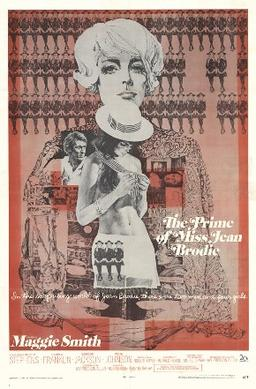
\includegraphics[scale=1.7]{a20220102ThePrimeofMissJeanBrody-img001.jpg} 
\end{wrapfigure}

\paragraph{Lady of Shalott}
In one scene Miss Brodie begins to recite by heart the \textit{Lady of Shalott} by Alfred, Lord Tennyson\footnote{See Section \ref{sec:LadyShallot} in this book.}. Elaine, the Lady of Charlotte, fell deeply in love with Lancelot, but that love was not reciprocated. She went down a river in a boat, as she slowly died. The water represents the soul and the lack of love is the death of the soul.

For a young woman, while there is a lack of love, her fantasies keep her soul alive. Elaine did experience real love, which could never be matched by a fantasy because it was unrequited. Hence, her soul slowly died.

We have to wonder, then, about how Miss Brodie experienced herself in that poem. She communicated solely in maxims and inspirational words that seem divorced from any real experience. Through art and poetry, she knew the concept of love but not the reality of love. True art, like the character in the \emph{Neverending Story}, asks us to participate in the soul of the artist, to enjoy his enjoyment.

As it dawns on Miss Brodie that she is past her prime, and she will forever be without love, there is nothing left but death. Her fate is unspecified in the movie.

\paragraph{Betrayal}
Sandy, her favorite student, the one with insight but no instinct according to Miss Brodie, soon sees through her teacher. She betrays Miss Brodie to the headmistress who have be looking for an excuse to terminate her. She also has an affair with the art teacher, perhaps to get back at Miss Brodie, but then leaves him when she realizes that he is still in love with Miss Brodie.

In our time, an affair between a 43 year old man and a high school student sounds creepy, but apparently it caused no stir in 1939. We get the impression that it was considered to be an honor to attract the attention of a male teacher.

\paragraph{Virginity}
For a woman, the question about losing her virginity usually has an import, but no logic as far as I can tell. For example, Elena, in My Brilliant Friend, loses it to an older man whom she despises, in a passionless act on the beach at night. Other stories are not much better.

The same story plays out in the decision to marry. Again, it often is a practical decision that must be made before losing her prime. One fellow told me about how he met his wife. He pestered her for six months until she finally yielded to him. He seemed quite proud about his persistence. I did not have the heart to explain to him that she was out and about for those six months looking for someone better. She only returned when she realized that he was the best she was going to do.

At some point she realizes that she is like the Lady of Shalott who has not found love; instead, she is waking up to a stranger every day. The esoteric teaching is that there is one woman for each man, who together form the Adam-Eve couple with is the return to the primordial state. In our current state of being, we find ourselves trapped in a web of relationships before we come to that awareness. Some fortunate ones escape from that web and find the one with whom there has been an entanglement from the beginning of the world.

\paragraph{Postscript on postmortem marriage}
Although marriage ends with death and there is no marrying in heaven, the idea persists that spouses will reunite in the afterlife. To be cynical, that is not necessarily an incentive for a lot of people. A more serious point is that there will be no physical bodies so souls will be fully exposed to each other. You may not even recognize your spouse in that case because you might not recognize her soul. The point is that it is necessary for a couple to share in each other's interiority. That, and only that, is the alchemical marriage.

\url{https://www.youtube.com/watch?v=IJZQz5U0el0}



\flrightit{Posted on 2022-01-02 by Cologero }

\begin{center}* * *\end{center}

\begin{footnotesize}\begin{sffamily}



\texttt{Alex on 2022-01-04 at 09:09 said: }

The act of marriage vows, living together for 20 years, arguing, making up, etc does not mean there will be any meeting of the two souls in the afterlife. Reasons for extending meetings into spirit life require some deep connection born of very real feelings which do not often follow from living together. Even if there is some communication between the living and dead it may be brief and not the pressing kind one witnesses with love. The dead are jealous of their new found freedom and checking in with the living is not their main priority.


\hfill

\texttt{Arthur Konrad on 2022-01-04 at 10:46 said: }

Alex, here is a question, I ask this as somebody who's got no idea.

If church marriage has no super-temporal meaning, which is to say, if marriage is until death do you part, then what's the difference between being married in a church and making religious vows, and doing the same at the city council? Also, since married persons definitely part at death, then why not before death? Why does the Church then oppose divorce at all, if marriage has got nothing to do with eternity? Does it all boil down then, to being loyal to each other in this life in a strictly corporal sense, for the sake of not doing bad (not hurting someone's feelings)? Is that what is holy and sanctified in the institution of marriage as the Church proscribes? I suppose that marriage with divine sanction would suggest something different – that spiritual loyalty precedes even this type of corporeal fidelity, in the sense that even adultery can be atoned for if one spouse's love for another prevails over temporary failings (I am aware of course, that most would not overlook adultery even in this case, but we know such stories)


\hfill

\texttt{Alex on 2022-01-04 at 18:53 said: }

Now, I think the practical reality of Christian marriage is to encourage the couple to stay together with the congregation supplying support on many levels and to remind them of a future in Heaven together with their loved ones. This support works to provide hope for a spiritual future which the county clerk cannot, making all the difference. We must use our discernment prior to marriage before setting sail on that white water expedition. Then once on the raft expect to get wet.


\end{sffamily}\end{footnotesize}
